\documentclass{report}

\usepackage{hyperref}

\usepackage{epstopdf}
\usepackage{amsmath}
\usepackage{amssymb}
\usepackage{subfig}
%\usepackage{multirow}
\usepackage[utf8]{inputenc}
\usepackage[T1]{fontenc}
\usepackage{standalone}
\usepackage{tikz}
\usepackage{tabularx}
\usepackage{float}
\usepackage[section]{placeins}
\usepackage{sverb}
\usepackage{import}
\usepackage{verbatim}
\usepackage{listings}
\usepackage{xcolor}

\graphicspath{{img/}}
\DeclareGraphicsExtensions{.pdf,.png,.jpg,.svg} %For pdflatex



\begin{document}

\begin{titlepage}
    \begin{center}
        \Huge
        \textbf{Przetwarzanie Obrazów Cyfrowych}
        \\ \vspace{1.5cm}
        \Large
        \textbf{Raport z ćwiczenia 2}        
    \end{center}
    \vspace{4.0cm}
    \Large
    Autor: \\
    Dawid Kania    
\end{titlepage}


\section*{
    zadanie 1: identyfikacja układu matrycy Bayer'a
}




\newcommand{\ww}{0.3} %zmienna używana jako parametr opisujące szerokość obrazu zdefiniowana poraz pierwszy w dokumencie


\begin{figure}[H]
    \captionsetup[subfloat]{justification=raggedright,singlelinecheck=false, position=bottom,labelformat=empty} %
    \subfloat[Obraz surowy          ]{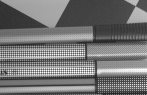
\includegraphics[width=\ww\linewidth]{../zad1/img1/img1_raw_.png }} \hfill%	
    \subfloat[GBRG                  ]{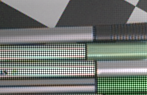
\includegraphics[width=\ww\linewidth]{../zad1/img1/img1_gbrg.png }} \hfill% wypełnenie
    \subfloat[GRBG                  ]{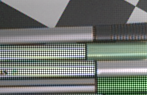
\includegraphics[width=\ww\linewidth]{../zad1/img1/img1_grbg.png }} \hfill
    \subfloat[Obraz wzorcowy - GT   ]{
\includegraphics[width=\ww\linewidth]{../zad1/img1/img1_gt__.png }} \hfill%
    \subfloat[BGGR (prawidłowy)     ]{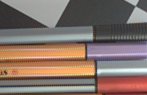
\includegraphics[width=\ww\linewidth]{../zad1/img1/img1_bggr.png }} \hfill%
    \subfloat[RGGB                  ]{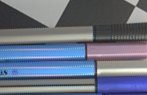
\includegraphics[width=\ww\linewidth]{../zad1/img1/img1_rggb.png }} 
    \caption{Identyfikacja układu matrycy Bayer'a. w tym przypadku prawidłowy jest układ BGGR} 
    \label{fig:porownanie1} %label który można wykorzystać w tekście za pomocą polecenia \ref{fig:porownanie1}
\end{figure}


\begin{figure}[H]
    \captionsetup[subfloat]{justification=raggedright,singlelinecheck=false, position=bottom,labelformat=empty} %
    \subfloat[Obraz surowy          ]{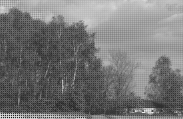
\includegraphics[width=\ww\linewidth]{../zad1/img07/img1_raw_.png }} \hfill%	
    \subfloat[GBRG                  ]{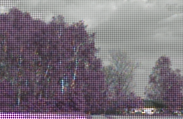
\includegraphics[width=\ww\linewidth]{../zad1/img07/img1_gbrg.png }} \hfill% wypełnenie
    \subfloat[GRBG                  ]{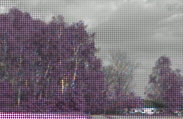
\includegraphics[width=\ww\linewidth]{../zad1/img07/img1_grbg.png }} \hfill
    \subfloat[Obraz wzorcowy - GT   ]{
\includegraphics[width=\ww\linewidth]{../zad1/img07/img1_gt__.png }} \hfill%
    \subfloat[BGGR (prawidłowy)     ]{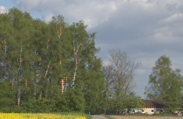
\includegraphics[width=\ww\linewidth]{../zad1/img07/img1_bggr.png }} \hfill%
    \subfloat[RGGB                  ]{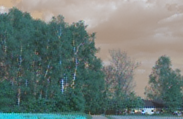
\includegraphics[width=\ww\linewidth]{../zad1/img07/img1_rggb.png }} 
    \caption{Identyfikacja układu matrycy Bayer'a. w tym przypadku prawidłowy jest układ BGGR} 
    \label{fig:porownanie1} %label który można wykorzystać w tekście za pomocą polecenia \ref{fig:porownanie1}
\end{figure}



\begin{figure}[H]
    \captionsetup[subfloat]{justification=raggedright,singlelinecheck=false, position=bottom,labelformat=empty} %
    \subfloat[Obraz surowy          ]{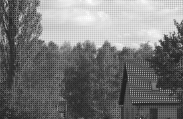
\includegraphics[width=\ww\linewidth]{../zad1/img08/img1_raw_.png }} \hfill%	
    \subfloat[GBRG                  ]{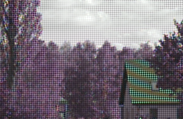
\includegraphics[width=\ww\linewidth]{../zad1/img08/img1_gbrg.png }} \hfill% wypełnenie
    \subfloat[GRBG                  ]{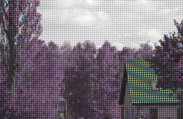
\includegraphics[width=\ww\linewidth]{../zad1/img08/img1_grbg.png }} \hfill
    \subfloat[Obraz wzorcowy - GT   ]{
\includegraphics[width=\ww\linewidth]{../zad1/img08/img1_gt__.png }} \hfill%
    \subfloat[BGGR (prawidłowy)     ]{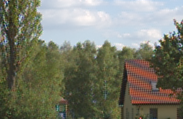
\includegraphics[width=\ww\linewidth]{../zad1/img08/img1_bggr.png }} \hfill%
    \subfloat[RGGB                  ]{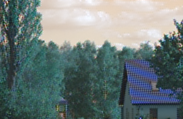
\includegraphics[width=\ww\linewidth]{../zad1/img08/img1_rggb.png }} 
    \caption{Identyfikacja układu matrycy Bayer'a. w tym przypadku prawidłowy jest układ BGGR} 
    \label{fig:porownanie1} %label który można wykorzystać w tekście za pomocą polecenia \ref{fig:porownanie1}
\end{figure}




\section*{Zadanie 2: Interpolacja metodą najbliższego sąsiada}

\begin{figure}[H]
    \captionsetup[subfloat]{justification=raggedright,singlelinecheck=false, position=bottom,labelformat=empty} %
    \subfloat[Obraz surowy 1        ]{\includegraphics[width=\ww\linewidth]{../zad2/img01/img1_orig.png }} \hfill%	
    \subfloat[NN 1 \\ (PSNR = 25.4501) ]{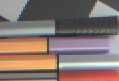
\includegraphics[width=\ww\linewidth]{../zad2/img01/img1_NN__.png }} \hfill% wypełnenie
    \subfloat[GT 1                  ]{\includegraphics[width=\ww\linewidth]{../zad2/img01/img1_reff.png }} \hfill
    \subfloat[Obraz surowy 2        ]{\includegraphics[width=\ww\linewidth]{../zad2/img08/img1_orig.png }} \hfill%
    \subfloat[NN 2 \\ (PSNR = 24.9508) ]{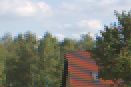
\includegraphics[width=\ww\linewidth]{../zad2/img08/img1_NN__.png }} \hfill%
    \subfloat[GT 2                  ]{\includegraphics[width=\ww\linewidth]{../zad2/img08/img1_reff.png }} 
    \caption{Prezentacja działania interpolacji metodą najbliższego sąsiada} 
    \label{fig:porownanie1} %label który można wykorzystać w tekście za pomocą polecenia \ref{fig:porownanie1}
\end{figure}



\begin{figure}[H]
    \captionsetup[subfloat]{justification=raggedright,singlelinecheck=false, position=bottom,labelformat=empty} %
    \subfloat[Obraz surowy 1        ]{
\includegraphics[width=\ww\linewidth]{../zad2/img22/img1_orig.png }} \hfill%	
    \subfloat[NN 1 \\ (PSNR = 23.9565) ]{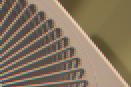
\includegraphics[width=\ww\linewidth]{../zad2/img22/img1_NN__.png }} \hfill% wypełnenie
    \subfloat[GT 1                  ]{\includegraphics[width=\ww\linewidth]{../zad2/img22/img1_reff.png }} \hfill
    \subfloat[Obraz surowy 2        ]{
\includegraphics[width=\ww\linewidth]{../zad2/img29/img1_orig.png }} \hfill%
    \subfloat[NN 2 \\ (PSNR = 24.9937) ]{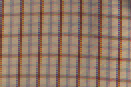
\includegraphics[width=\ww\linewidth]{../zad2/img29/img1_NN__.png }} \hfill%
    \subfloat[GT 2                  ]{\includegraphics[width=\ww\linewidth]{../zad2/img29/img1_reff.png }} 
    \caption{Prezentacja działania interpolacji metodą najbliższego sąsiada} 
    \label{fig:porownanie1} %label który można wykorzystać w tekście za pomocą polecenia \ref{fig:porownanie1}
\end{figure}


\section*{Zadanie 3: Interpolacja biliniowa}

\begin{figure}[H]
    \captionsetup[subfloat]{justification=raggedright,singlelinecheck=false, position=bottom,labelformat=empty} %
    \subfloat[Obraz surowy 1               ]{\includegraphics[width=\ww\linewidth]{../zad3/img01/img1_orig.png }} \hfill%	
    \subfloat[Biliniowa 1 \\ (PSNR = 29.1382) ]{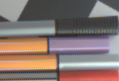
\includegraphics[width=\ww\linewidth]{../zad3/img01/img1_NN__.png }} \hfill% wypełnenie
    \subfloat[GT 1                         ]{\includegraphics[width=\ww\linewidth]{../zad3/img01/img1_reff.png }} \hfill
    \subfloat[Obraz surowy 2               ]{\includegraphics[width=\ww\linewidth]{../zad3/img08/img1_orig.png }} \hfill%
    \subfloat[Biliniowa 2 \\ (PSNR = 27.931)  ]{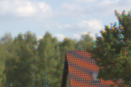
\includegraphics[width=\ww\linewidth]{../zad3/img08/img1_NN__.png }} \hfill%
    \subfloat[GT 2                         ]{\includegraphics[width=\ww\linewidth]{../zad3/img08/img1_reff.png }} 
    \caption{Prezentacja działania interpolacji biliniowej} 
    \label{fig:porownanie1} %label który można wykorzystać w tekście za pomocą polecenia \ref{fig:porownanie1}
\end{figure}



\begin{figure}[H]
    \captionsetup[subfloat]{justification=raggedright,singlelinecheck=false, position=bottom,labelformat=empty} %
    \subfloat[Obraz surowy 1                ]{
\includegraphics[width=\ww\linewidth]{../zad3/img22/img1_orig.png }} \hfill%	
    \subfloat[Biliniowa 1 \\ (PSNR = 29.1615)  ]{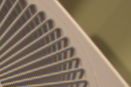
\includegraphics[width=\ww\linewidth]{../zad3/img22/img1_NN__.png }} \hfill% wypełnenie
    \subfloat[GT 1                          ]{\includegraphics[width=\ww\linewidth]{../zad3/img22/img1_reff.png }} \hfill
    \subfloat[Obraz surowy 2                ]{
\includegraphics[width=\ww\linewidth]{../zad3/img29/img1_orig.png }} \hfill%
    \subfloat[Biliniowa 2 \\ (PSNR = 30.2622)  ]{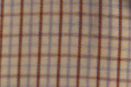
\includegraphics[width=\ww\linewidth]{../zad3/img29/img1_NN__.png }} \hfill%
    \subfloat[GT 2                          ]{\includegraphics[width=\ww\linewidth]{../zad3/img29/img1_reff.png }} 
    \caption{Prezentacja działania interpolacji biliniowej} 
    \label{fig:porownanie1} %label który można wykorzystać w tekście za pomocą polecenia \ref{fig:porownanie1}
\end{figure}



\newpage

\section*{Kody Programów}


\definecolor{codegreen}{rgb}{0,0.6,0}
\definecolor{codegray}{rgb}{0.5,0.5,0.5}
\definecolor{codepurple}{rgb}{0.58,0,0.82}
\definecolor{backcolour}{rgb}{0.95,0.95,0.92}

\lstdefinestyle{mystyle}{
    backgroundcolor=\color{backcolour},   
    commentstyle=\color{codegreen},
    keywordstyle=\color{magenta},
    numberstyle=\tiny\color{codegray},
    stringstyle=\color{codepurple},
    basicstyle=\ttfamily\footnotesize,
    breakatwhitespace=false,         
    breaklines=true,                 
    captionpos=b,                    
    keepspaces=true,                 
    numbers=left,                    
    numbersep=5pt,                  
    showspaces=false,                
    showstringspaces=false,
    showtabs=false,                  
    tabsize=2
}


\lstset{style=mystyle}

\subsection*{zad1.m               } \lstinputlisting[language=Octave]{../Matlab/zad1.m              } \newpage
\subsection*{zad2.m               } \lstinputlisting[language=Octave]{../Matlab/zad2.m              } \newpage
\subsection*{zad3.m               } \lstinputlisting[language=Octave]{../Matlab/zad3.m              } \newpage
\subsection*{demosaic\_nearest.m  } \lstinputlisting[language=Octave]{../Matlab/demosaic_nearest.m  } \newpage
\subsection*{demosaic\_bilinear.m } \lstinputlisting[language=Octave]{../Matlab/demosaic_bilinear.m } \newpage
\subsection*{cropImage.m          } \lstinputlisting[language=Octave]{../Matlab/cropImage.m         } \newpage

 





\end{document}